%
% File: chap03.tex
% Author: Your name
% Description: Results 
%
\let\textcircled=\pgftextcircled
\chapter{Methodology}
\label{chap:example}


%%%%%%%%%%%%%%%%%%%%%%%%%%%%%%%%%%%%%%%%%%%%%%%%%%%%%%%%%%%%%%%%%%%%%%
\section{Dataset}
\initial{I}n this section, we describe the data gathering process. In this paper, we use the Eikon Refinitiv database. We extract all available bond data between January 01, 2008 and September 26, 2022 and follow the literature by filtering bonds by issue amount ($\geq$ USD 500 million)\footnote{This contrasts with \cite{loffler2021drivers}'s study, which applies the filter at USD 200 million.} \citep[p. 8]{caramichael2022green}, coupon type (fixed rate only), and time to maturity (>1 year). The first and third criteria are relevant to bypass controlling for liquidity premia in the analysis. Similarly, restricting the data to fixed coupon bonds reduces complexity and also mitigates later issues of unobservable confounding due to uncertainty \citep[p. 128]{gianfrate2019green}.

\begin{table}[h!]
\caption{Eikon Refinitiv Search Criteria}
\small
\begin{tabular}{ll} \hline
\hline
\textbf{Criteria} & \textbf{Description} \\ \hline
Issuance Date & 01. Jan 2008 - 26 Sep 2022 \\
Sustainable Finance Flag & True/False \\
Transaction Status & Live, Redeemed \\
Principal Amount & $\geq$ USD 500'000'000 \\
Issue Type & \begin{tabular}[c]{@{}l@{}}Agency, Supranational, Sovereign, Emerging Market Corporate, \\ Federal Credit Agency, High Yield Corporate, Investment Grade Corporate\end{tabular} \\
Coupon Type & Fixed Rate \\
Private Placement Flag & False \\ \hline
\end{tabular}
\end{table}

%%%%%%%%%%%%%%%%%%%%%%%%%%%%%%%%%%%%%%%%%%%%%%%%%%%%%%%%%%%%%%%%%%%%%%
\subsection{Variables}
%%%%%%%%%%%%%%%%%%%%%%%%%%%%%%%%%%%%%%%%%%%%%%%%%%%%%%%%%%%%%%%%%%%%%%

With the exception of two variables, all variables described in Table \ref{vardesc} were taken from the Eikon Refinitiv deal screen database. These two variables are ESG bond type and seniority. We collected them by accessing a database through the formula builder of the Refinitiv Excel plugin using the ISINs of the bonds. As for ratings, we could only obtain this information from Moody's. Unfortunately, ratings from S\&P and Fitch were not available under the license. Finally, our universe data set consists of 14 potential covariates, an outcome variable, i.e., the offer yield to maturity, and a treatment variable, i.e., the green flag.

\begin{table}[!h] \centering 
  \caption{Variable Description} 
  \label{vardesc}
  \begin{adjustbox}{width=\columnwidth,center}
\begin{tabular}{@{\extracolsep{5pt}}lccp{10cm}p{3cm}} 
\\[-1.8ex]\hline 
\hline \\[-1.8ex] 
Variable name & \multicolumn{1}{c}{Binary} & \multicolumn{1}{c}{Type} & Description \\ 
\hline \\[-1.8ex] 
Issue Date & No & C & Date of Issuance; Years: 2008-2022 \\
Maturity Date & No & C &  Date of Maturity\\
Time to Maturity (Days) & No & C & Date of Maturity $-$ Date of Issuance (in days)\\
Issuer & Yes & C & Name of Issuer \\
Issuer Type & Yes & C & Type of Issuer: Dummy equal to 1 (Public sector) for bonds issued by agency, supranational, sovereign or federal credit agency. Otherwise 0 (Private sector) for bonds issued by investment grade corporates, emerging market corporates or high yield corporates \\
Issued Amount & No & C & Amount of Issuance\\
TRBC Economic Sector & Yes & C & Academic \& Educational Services, Basic Materials, Consumer Cyclicals, Consumer Non-Cyclicals, Energy, Financials, Government Activity, Healthcare, Industrials, Institutions, Associations \& Organizations, Real Estate, Technology, Utilities \\
Coupon Rate & Yes & C & Coupon in Percentage\\
New Issues Rating (Moody's) & Yes & C & Rating conversion: AAA = Aaa; AA = Aa1, Aa2, Aa3; A = A1, A2, A3; BBB = Baa1, Baa2, Baa3; BB = Ba1, Ba2, Ba3; B = B1, B2, B3; CCC = Caa1, Caa2, Caa3\\
Currency & Yes & C & Australian Dollar (AUD), Braziliean Real (BRL), Canadian Dollar (CAD), Chilean Peso (CLP), Chinese Yuan Renminbi (CNY), Colombian Peso (COP), Croation Kuna (HRK), Euro (EUR), Great Britain Pound (GBP), Hong Kong Dollar (HKD), Japanese Yen (JPY), Kazhakstan Tenge (KZT), Mexican Peso (MXN), New Zealand Dollar (NZD), Norwegian Krone (NOK), Peruvian Nuevo Sol (PEN), Philippine Peso (PHP), Russan New Ruble (RUB), Singapore Dollar (SGD), Swedish Krona (SEK), Swiss Franc (CHF), Thai Baht (THB), New Turkish Lira (TRY), U.S. Dollar (USD), Uruguayan Peso Uruguayano (UYU)\\
Guarantor & Yes & C &  Dummy equal to 1 if bond is secured by any kind of the following credit enhancement types: Guaranteed by an Entity, Insured, Keep Well Agreement, Letter of Credit, Line of Credit, Liquidity Agreement, Purchase Agreement, State Sponsored or Support Agreement; 0 else\\
Coupon Payment Frequency & Yes & C & Annual Coupon, Semi Annual Coupon, Quarterly, Monthly \\
Seniority & Yes & C & First-Lien Loan, First Mortgage, First Refunding Mortgage, Second-Lien Loan, Junior Subordinated, Senior Secured Mortgage, Refunding Mortgage, Senior Secured, Senior Unsecured, Senior Non-Preferred, Senior Preferred, Senior Secured, Subordinated Unsecured, Subordinated Secured\\
Offer Yield to Maturity & No & O & Yield offered to Investors at Issuance in Percentage \\
ESG Bond Type & Yes & C & CBI aligned green bond, CBI certified green bond, No ESG, Not disclosed, Self-labelled\\
Green Flag & Yes & T & Dummy equal to 1 if green bond; 0 else\\
\hline \\[-1.8ex] 
\end{tabular} 
\end{adjustbox}
\vspace{1ex}

     {\raggedright Type: C = Covariate; O = Outcome; T = Treatment \par}
\end{table}
%%%%%%%%%%%%%%%%%%%%%%%%%%%%%%%%%%%%%%%%%%%%%%%%%%%%%%%%%%%%%%%%%%%%%%
\subsection{Data Cleaning}
Table \ref{cleaning} describes the cleaning process. We did our best to minimize missing green bond values by manually adding values from the Bloomberg database. The list of ISINs for which we have added this data can be found in the appendix (\ref{appE}). Moreover, we found a highly implausible value of the outcome variable (offer yield to maturity) amounting to 99.852\% which we adjusted for the true value. Our final sample, which we refer to as our universe, consists of 1'065 green bonds and 11'331 brown bonds. Based on this dataset, we form three subsamples, which we will explain in more detail after describing the variables in the next section.

\begin{table}[h!]
\caption{Data Cleaning Process}
\label{cleaning}
\begin{adjustbox}{center}
\begin{tabular}{llll}
\hline
 \hline
 & \textbf{\# Green Bonds} & & \textbf{\# Brown Bonds} \\ \hline
Total & 1'686 & Total & 37'076 \\ 
Missing Issuance Date & -126 & Total Missing Values & -25'745 \\ 
Perpetual Maturity & -2 \\ 
Time to Maturity \textless 1 year & -78 \\ 
Missing Yield at Issuance & -13 \\ 
Duplicates & -49 \\ 
Missing Moody's Rating & -317 \\ \hline
& \bfseries{1'065} & & \bfseries{11'331} \\ \cline{2-2} \cline{4-4}
\end{tabular}
\end{adjustbox}
\end{table}
%%%%%%%%%%%%%%%%%%%%%%%%%%%%%%%%%%%%%%%%%%%%%%%%%%%%%%%%%%%%%%%%%%%%%%
\subsection{Subset}

To leverage the potential of our dataset and to assess the research question more precisely in terms of robustness, we formed three subsamples. First, based on our original so-called universe dataset, we constructed a subsample that includes only issuers that have issued both green and conventional bonds. This eliminates the need to control for each issuer in the analysis. Second, we drew two different subsamples based on the first subsample. First, to further control for liquidity issues due to small bond markets, we included bonds denominated in euros and U.S. dollars in the subsample. These two currencies account for 90\% of the total green bond market. On the other hand, we drew a subsample based on the variable "ESG bond type" to include only green bonds that are either aligned or certified by the CBI. This allows us to analyze whether these bonds are valued differently. These types of bonds account for 58\% of the green bonds in our first subsample.

\newpage
%%%%%%%%%%%%%%%%%%%%%%%%%%%%%%%%%%%%%%%%%%%%%%%%%%%%%%%%%%%%%%%%%%%%%%


%%%%%%%%%%%%%%%%%%%%%%%%%%%%%%%%%%%%%%%%%%%%%%%%%%%%%%%%%%%%%%%%%%%%%%
\section{Methods}
%%%%%%%%%%%%%%%%%%%%%%%%%%%%%%%%%%%%%%%%%%%%%%%%%%%%%%%%%%%%%%%%%%%%%%

\subsection{Causal Inference Framework}

We start by defining some common notations. Each unit in the dataset will be represented by:

\begin{enumerate}
    \item \textbf{$X_{i}$} : is a $K$-component vector of features, i.e. covariates, known not to be affected by the treatment;
    \item $D_{i} \in\{0,1\}$ : is a binary variable indicating whether the individual was treated (1) or not (0);
    \item $Y_{i}^{\text {obs }} \in \mathbb{R}$ : is the observed outcome for that individual.
\end{enumerate}

To isolate the causal effect, one must look for a convincing ceteris paribus comparison. This is why causal statements involve counterfactual comparisons, i.e., what would have been observed for the same unit under a different treatment. To express this mathematically, this study uses the notion of potential outcome, as first formulated by \citet{rubin1974estimating}:

\begin{enumerate}
    \item $Y_{i}(1)$ : the outcome unit $i$ would attain if they received the treatment;
    \item $Y_{i}(0)$ : the outcome unit $i$ would attain if they were part of the control group.
\end{enumerate}

Obviously, we can only observe one of these two potential outcomes for each unit. Indeed, we can observe either the realization of $\left(X_{i}, Y_{i}(0)\right)$ for the control units or $\left(X_{i}, Y_{i}(1)\right)$ for the treated units, while the other potential outcome is always unobservable. This is what is called the "fundamental problem of causal inference". The goal of causal inference is therefore to predict these counterfactuals, in order to estimate the average treatment effect as an expectation of the difference between the two:

\begin{equation}
    \text{ATE} = \mathrm{E}[Y_{i}(1)-Y_{i}(0)]
\end{equation}

If one wishes to estimate the treatment effect for specific subgroups within a population, it can be obtained by conditioning on a set of covariates. When the treatment effect is heterogeneous with respect to these covariates, this heterogeneity can be captured by (the expectation of) the conditional distribution of the random variable $Y_{i}(1) - Y_{i}(0)$ on the vector of covariates X. This conditional expectation is called the conditional average treatment effect, or CATE and is expressed as:

\begin{align}
    \text{CATE}(x) &= \mathrm{E}[Y_{i}(1)-Y_{i}(0) \mid X=x] \\
    &= \mathrm{E}[Y_{i}(1) \mid X_{i}=x]-\mathrm{E}[Y_{i}(0) \mid X_{i}=x] \nonumber \\
    &= \mathrm{E}[Y_{i} \mid X_{i}=x, D=1]-\mathrm{E}[Y_{i} \mid X_{i}=x, D=0] \nonumber \\
    &= \mu_1(x)-\mu_0(x) \nonumber
\end{align}

However, the data alone are not sufficient to predict the counterfactual outcome. To identify the effects of interest, we require a set of identification assumptions. These assumptions depend on a particular study design. In our case, the data are observational, as the treatment was not randomly assigned to the study population, but only observed. Thus, the selection-on-observables design comes to the fore. In this setting, it is very probable that companies that issue green bonds are systematically different from companies that do not issue green bonds. To account for this unequal comparison, the selection-on-observables strategy assumes that we observe and adjust for all relevant confounders, i.e., all covariates $X_i$ that jointly affect both treatment $D_i$ and potential outcomes $Y_{i}(0)$ and $Y_{i}(1)$.

\begin{enumerate}[font=\bfseries]
    \item \textbf{Assumption: Unconfoundedness}. This condition requires that potential outcomes are conditionally independent of treatment for any given value of the confounding variables. In other words, once we condition on the observable characteristics, the treatment assignment is independent of how each individual would respond to the treatment. Mathematically, this can be expressed as follows:
    \begin{equation}
        Y_{i}(1), Y_{i}(0) \perp D_{i} \mid X_{i}=x.
    \end{equation}
    where $\perp$ stands for independence. 
    The assumption of unconfounded assignment is always valid in randomized experiments, or when all confounding variables, i.e., variables that jointly influence the outcome Y and the treatment, are observable and included in the model. Finally, it is also known as the conditional independence assumption (CIA).
    \item \textbf{Assumption: Overlap or Common Support}. For any given value of the confounding variable, one unit could potentially be observed in both treatments. Indeed, to estimate the treatment effect for a unit with particular characteristics $X_i=x$, we must ensure that we can observe treated and untreated individuals with these same characteristics. Since causal effects are based on the comparison of units with the same characteristics but different treatments, they ensure that such units exist.
    Mathematically, it can be written as: 
    \begin{equation}
        \forall x \in \operatorname{supp}(X), \quad 0<P(X=1 \mid X=x)<1.
    \end{equation}
    In other words, we need to ensure that any observation, regardless of its covariate values, has a chance of being assigned to either the treated or control group.
    \item \textbf{Assumption: SUTVA}. This assumption is known as the stable unit treatment value assumption and states that the observed treatment value for one unit is independent of the treatment exposure for other units, ruling out any general equilibrium or spillover effects between treated and control units. Mathematically, it can be expressed as follows:
    \begin{equation}
    Y_i=W_i \cdot Y_i(1)+\left(1-W_i\right) \cdot Y_i(0).
    \end{equation}
    Moreover, this assumption also implies the condition that there are no hidden variations in treatment for each unit.
    \item \textbf{Assumption: Exogeneity}. This last assumption requires that the covariates are not influenced by the treatment, again mathematically formulated as follows: 
    \begin{equation}
    X_i(0)=X_i(1).
    \end{equation}
\end{enumerate}


\subsection{Causal Machine Learning: Causal Forest}
Causal Forests build on the idea of Random Forests (\cite{breiman2001random}). These machine learning methods seem remarkably effective in prediction contexts. However, good performance in prediction does not necessarily mean good performance in estimation or in inference on "causal" parameters. To enable these methods for a causal framework, scientists have developed techniques consistent with theory to avoid bias in estimation. Our paper builds on the methods developed by \cite{athey2019generalized} and \cite{wager2018estimation}. These causal forests are a specialization of the generalized random forest algorithm with the goal of estimating the conditional average treatment effect (CATE). Its implementation is motivated by the R-learner \cite{niewager}, i.e., a meta-algorithm using the idea of orthogonalization to cancel any feature selection bias (regularization bias) \citep[p. 5]{athey2019generalized}. In the following paragraphs we will describe the basic idea of this method.

The idea of Causal Forest is to construct and average many different deep Causal Trees. While deep trees often have low bias but high variance in their prediction, averaging over many trees largely reduces the variance while keeping the bias low. To ensure that individual trees are sufficiently different, each tree is created from only a random subsample of observations and a subsample of covariates. When each individual tree in the forest is estimated honestly, the causal forest estimates are unbiased and have valid confidence intervals. A method is honest if it uses one subset of the data to estimate the model parameters and another subset to produce estimates based on those estimated parameters. The Causal Forest allows us first to estimate the heterogeneity of causal effects and then to make inferences about the magnitude of differences in treatment effects, i.e., to test hypotheses about differences in effects across subpopulations.

In mathematical terms, suppose that we have a training set $\left\{\left(X_i, Y_i, W_i\right)\right\}_{i=1}^n$, a test point $x$, and a tree predictor $T$:
$$
\hat{\tau}(x)=T\left(x ;\left\{\left(X_i, Y_i, W_i\right)\right\}_{i=1}^n\right)
$$
We can replace the tree predictor by building and averaging many different trees $T^*$:
$$
\hat{\tau}(x)=\frac{1}{B} \sum_{b=1}^B T_b^*\left(x ;\left\{\left(X_i, Y_i, W_i\right)\right\}_{i=1}^n\right)
$$

In addition to this "ensemble" way of thinking, where a Random Forest prediction is an average of the predictions of the individual trees, we can also think of Random Forests as an adaptive kernel method \citep[p. 5]{atheywagerapplication}:

\begin{equation}
\hat{\tau}(x)=\sum_{i=1}^n \alpha_i(x) Y_i, \quad 
\alpha_i(x)=\frac{1}{B} \sum_{b=1}^B T_b^*\left(x ;\left\{\left(X_i, W_i\right)\right\}_{i=1}^n\right),
\end{equation}

where $\alpha_i(x)$ is a data-adaptive kernel that measures how often each training sample falls in the same leaf as the test point x \citep[p. 5]{atheywagerapplication}. This weighting approach is illustrated in Figure \ref{rfill}.

\begin{figure}
    \centering
    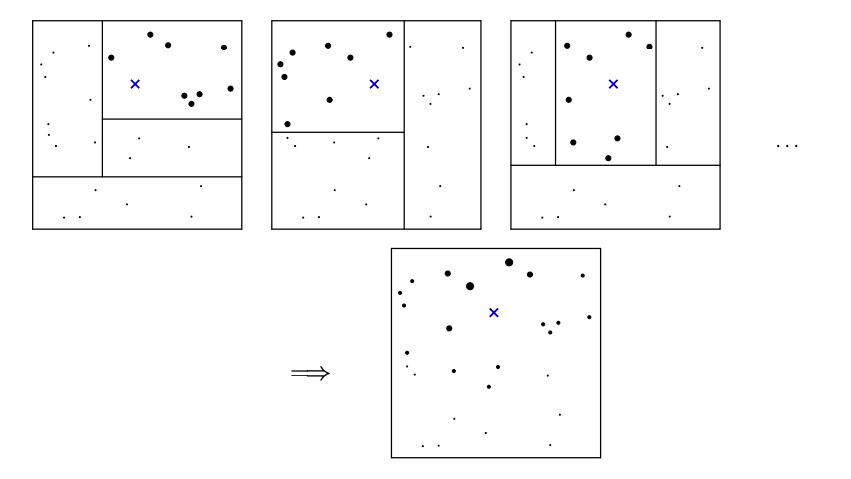
\includegraphics[scale=0.5]{chinchilab-template/chapters/chapter03/Causal Forest.png}
    \caption{Illustration of the Random Forest weighting function. Reprinted from \citeauthor{athey2019generalized} [2019, p. 6].}
    \label{rfill}
\end{figure}

The implementation of the Causal Forest method in R is provided by the \textit{grf} (generalized random forest) package. For the estimation of the average treatment effect (ATE), the package applies the augmented inverse probability weighting (AIPW) method, which is a doubly-robust estimator. Using the propensity score $e(x)=P\left[W_i \mid X_i=x\right]$ and the response function $m(x)=E\left[Y_i \mid X_i=x\right]$, the ATE is consistent when either function is consistent. Further, if the conditional average treatment function is constant, i.e. $\tau(x) = \tau$ for all $x \in \mathcal{X}$, we can write the estimator mathematically as follows \citep[p. 4]{atheywagerapplication}:

\begin{equation}
\hat{\tau}=\frac{\frac{1}{n} \sum_{i=1}^n\left(Y_i-\hat{m}\left(X_i\right)\right)\left(W_i-\hat{e}\left(X_i\right)\right)}{\frac{1}{n} \sum_{i=1}^n\left(W_i-\hat{e}\left(X_i\right)\right)^2}
\end{equation}

Finally, beyond the assumption presented in the previous subsection, this method requires that the data are independently and identically distributed (i.i.d) (\citep[p. 4]{atheywagerapplication}.

\subsection{Matching}
Matching is an increasingly popular method for controlling observed confounding variables when estimating causal effects in non-experimental studies. The purpose is to guarantee that there are no large differences in the distribution of the observed covariates in the treatment and comparison groups, as would be the case if a randomized experiment were conducted \citep[p. 2]{stuart2008using}.
Thus, if the distributions are sufficiently similar, this should result in little bias in the estimated treatment effect [p. 9].
In an optimal scenario, one would require perfect matches between treatment and comparison groups. Although such a method, i.e., exact matching, exists, it is rarely feasible because it would require a data set with a vast number of observations and relatively few confounding variables \citep[p. 602]{bekes2021data}. In the following subsections, we briefly summarize the propensity score matching approach.

Prior to this, it is worth mentioning the four steps of implementing matching methods, as described by \citet[pp. 5ff.]{stuart2010matching}:

\begin{enumerate}
    \item Defining "closeness": the distance measure used to calculate whether a treated observation closely matches an untreated observation. (E.g., Exact, Mahalanobis, Propensity Score etc.);
    \item Implementing a matching method. (E.g. Nearest neighbour, Subclassification etc.);
    \item Quality Assessment (i.e. balance checks): possibly re-iterating step (1) and (2) until a well-matched (well-balanced) sample is obtained;
    \item Analysis of the outcome and estimation of treatment effect.
\end{enumerate}

\subsubsection*{Propensity Score Matching}
As the name suggests, the basic idea of this method is to estimate a propensity score, i.e., a single scalar, defined mathematically as follows:

\begin{equation}
    e_i (X_i) = Pr[D_i = 1 | X_i]
\end{equation}

The equation reads: the propensity score is the conditional probability of being treated for each observation in the data, given all confounder variables. Estimating such a probability model is straightforward, using either a logit or probit model. To match the treated observations and the control observations based on their similarity in propensity scores, one can use the most widely used matching procedure called nearest neighbor matching \citep[p. 604]{bekes2021data}. In its most basic form, the so-called 1:1 nearest neighbor matching algorithm selects the control observation $j$ with the smallest distance between it and the treated observation $i$ for each treated observation. Mathematically, this can be expressed as follows \citep[p. 936]{wooldridge2010econometric}:

\begin{equation}
    h(i) = \text{argmin}_h |\hat{e}(x_j)-\hat{e}(x_i)|
\end{equation}


However, this approach may result in poor matches if, for instance, no control observation has a similar propensity score to a particular treatment observation \citep[p. 10]{stuart2010matching}. In such a situation, as described by the matching process of \citet{stuart2010matching} above, one should opt to iteratively choose different covariates for matching or use a different probability model until the balance checks are well-satisfied. 
To sum up, the propensity score matching approach suffers from some pitfalls: (1) It cannot guarantee any level of imbalance or model dependence reduction, (2) the dimensionality reduction by estimating a single scalar violates the congruence principle \citep[p. 2]{iacus2012causal}.

